\section{Aneks: dodatkowe wyniki analizy graficznej}

W niniejszym aneksie zamieszczono dodatkowe wizualizacje wykorzystane podczas wstępnej analizy danych. Obejmują one wykresy pudełkowe, macierz korelacji, rozkłady cech dla całego zbioru oraz rozkłady cech wyznaczone osobno dla poszczególnych klas, a także wykres typu \textit{pairplot}.

\begin{figure}[!htbp]
    \centering
    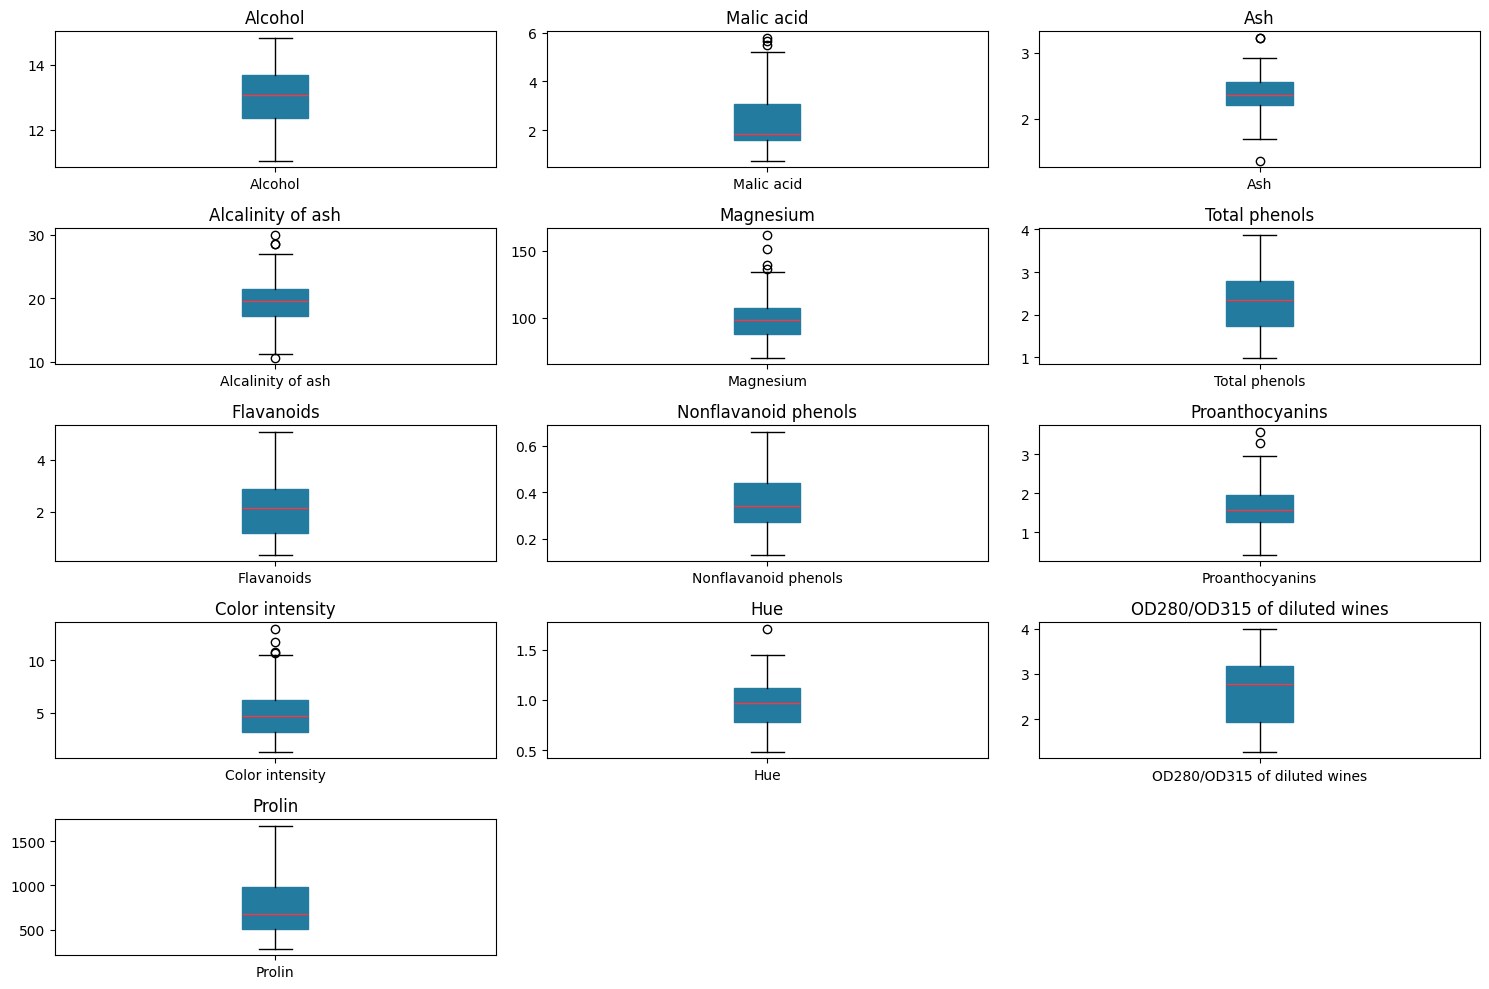
\includegraphics[width=0.9\textwidth]{figures/boxplotpng.png}
    \caption{Boxplots for the considered input variables in the dataset.}
    \label{fig:boxplots}
\end{figure}

\begin{figure}[!htbp]
    \centering
    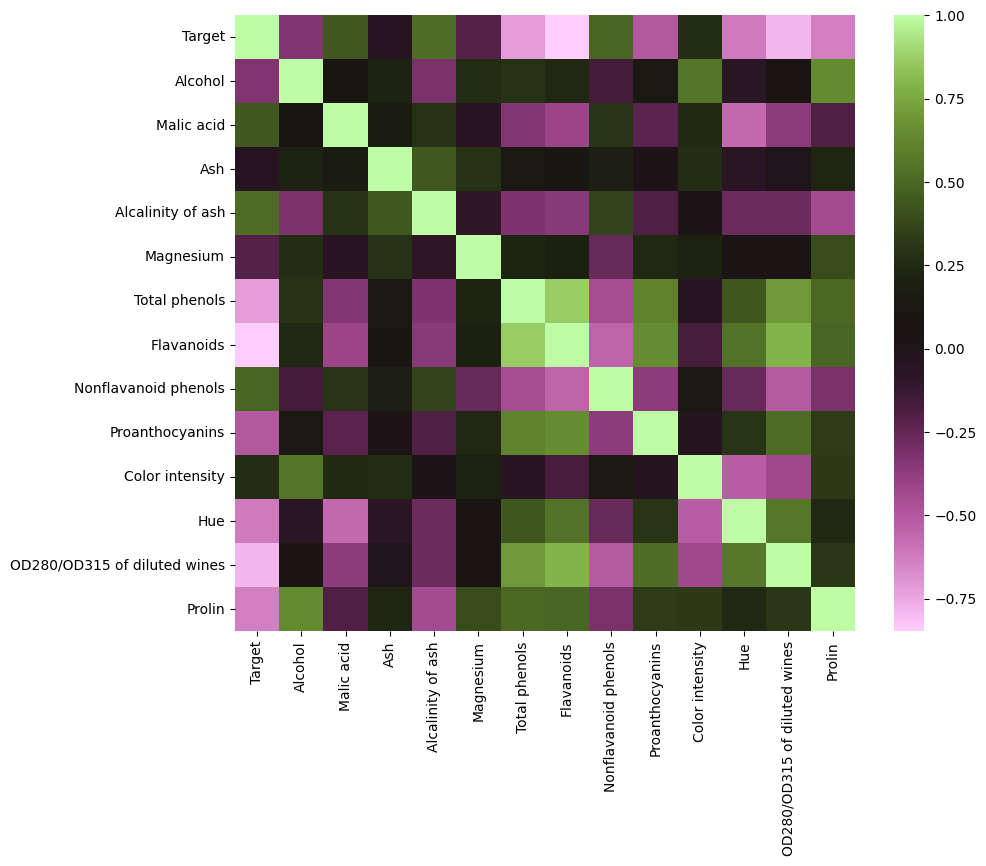
\includegraphics[width=0.85\textwidth]{figures/corelation_matrix.png}
    \caption{Correlation matrix for the considered input variables.}
    \label{fig:correlation_matrix}
\end{figure}

\begin{figure}[!htbp]
    \centering
    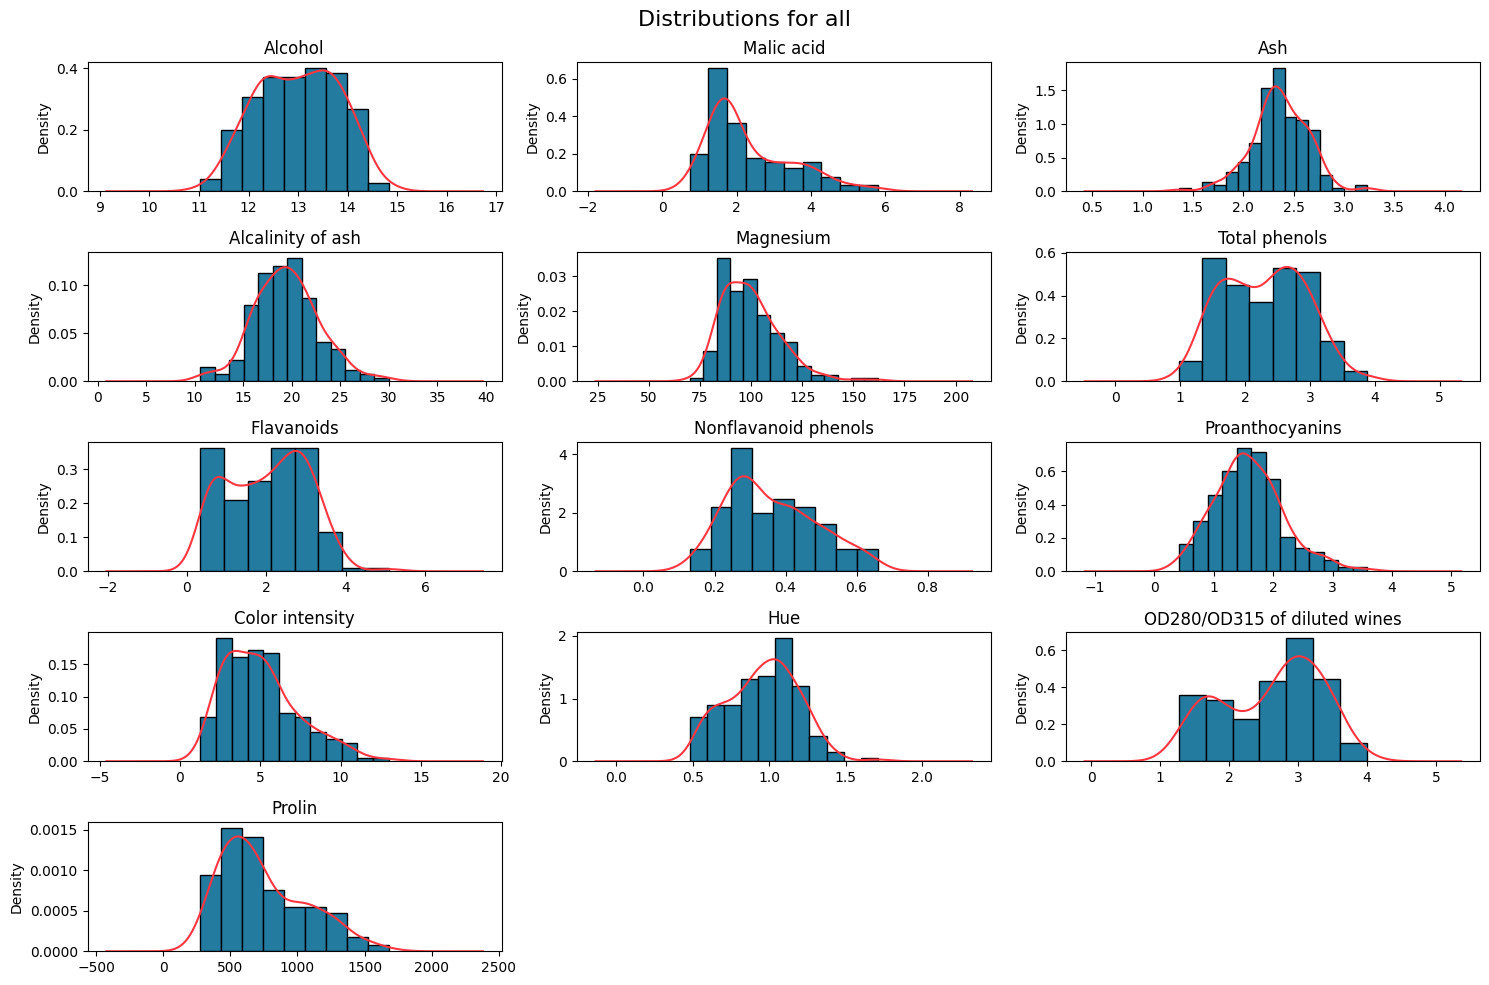
\includegraphics[width=\textwidth]{figures/Distribiutions_all.png}
    \caption{Distributions of the considered variables for the entire dataset.}
    \label{fig:distributions_all}
\end{figure}

\begin{figure}[!htbp]
    \centering
    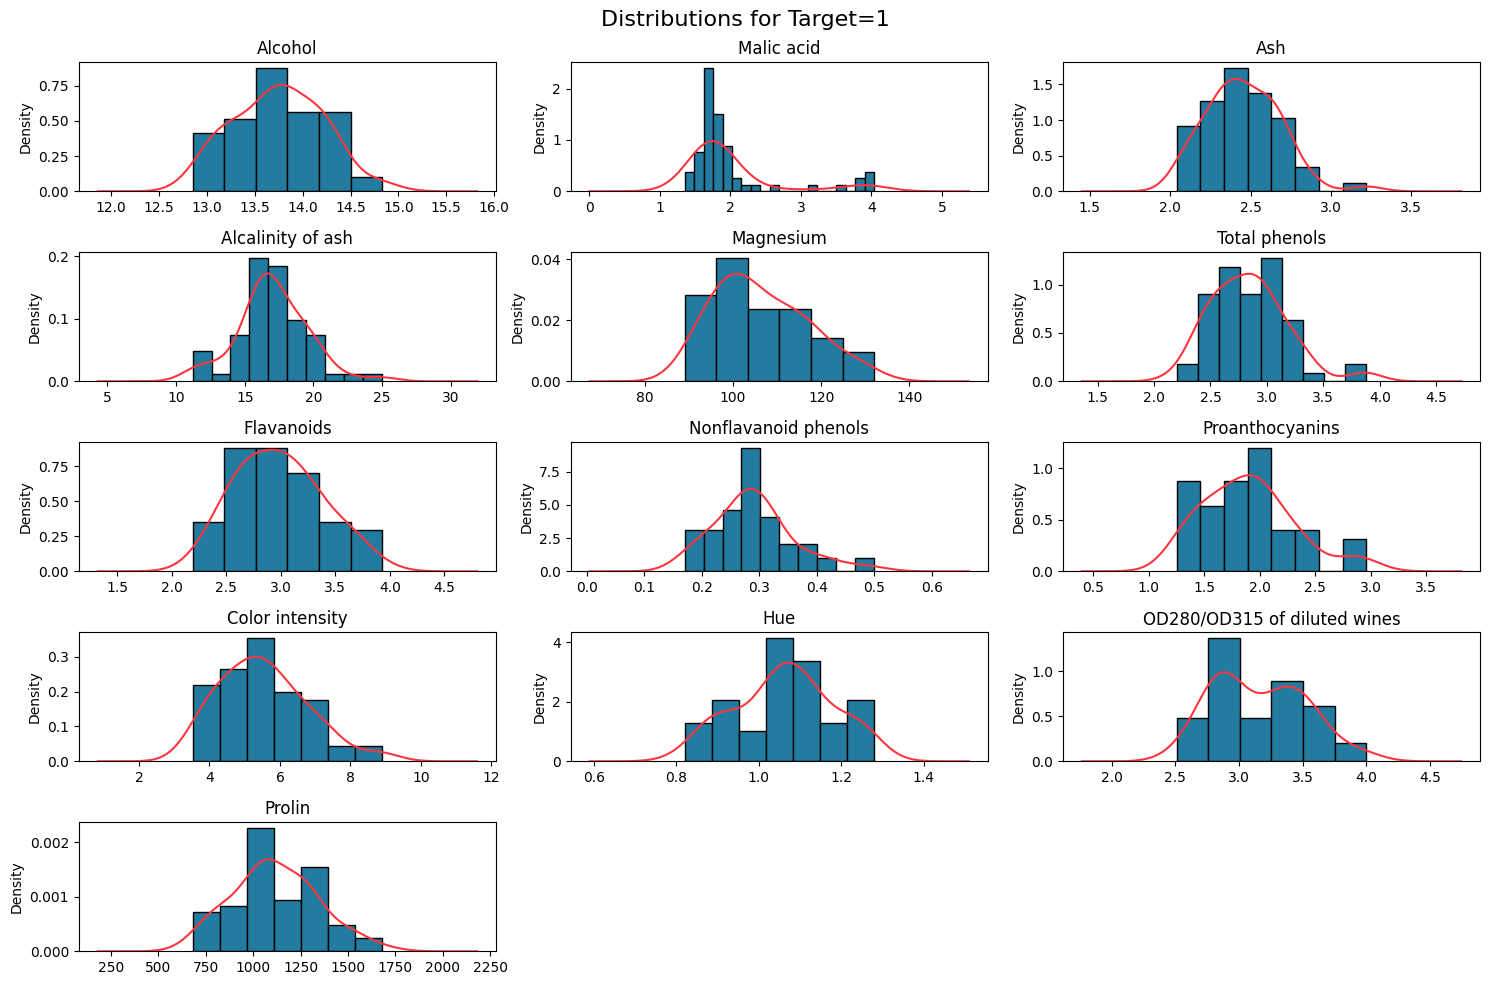
\includegraphics[width=\textwidth]{figures/Distribiutions_target1.png}
    \caption{Distributions of the considered variables for observations belonging to class 1.}
    \label{fig:distributions_target1}
\end{figure}

\begin{figure}[!htbp]
    \centering
    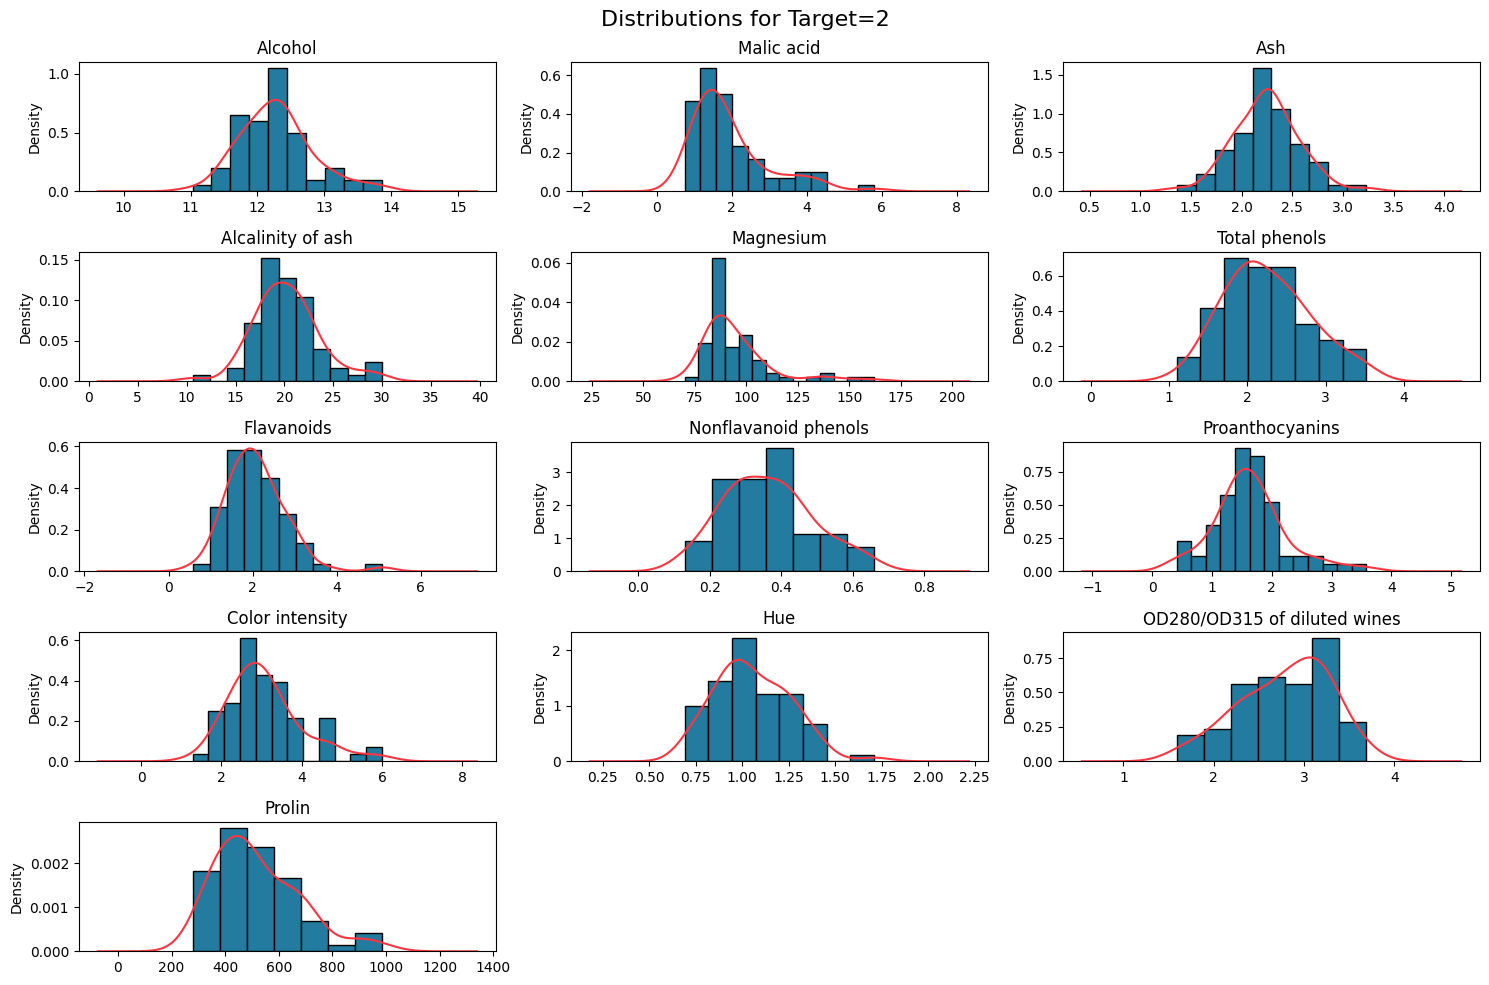
\includegraphics[width=\textwidth]{figures/Distribiutions_target2.png}
    \caption{Distributions of the considered variables for observations belonging to class 2.}
    \label{fig:distributions_target2}
\end{figure}

\begin{figure}[!htbp]
    \centering
    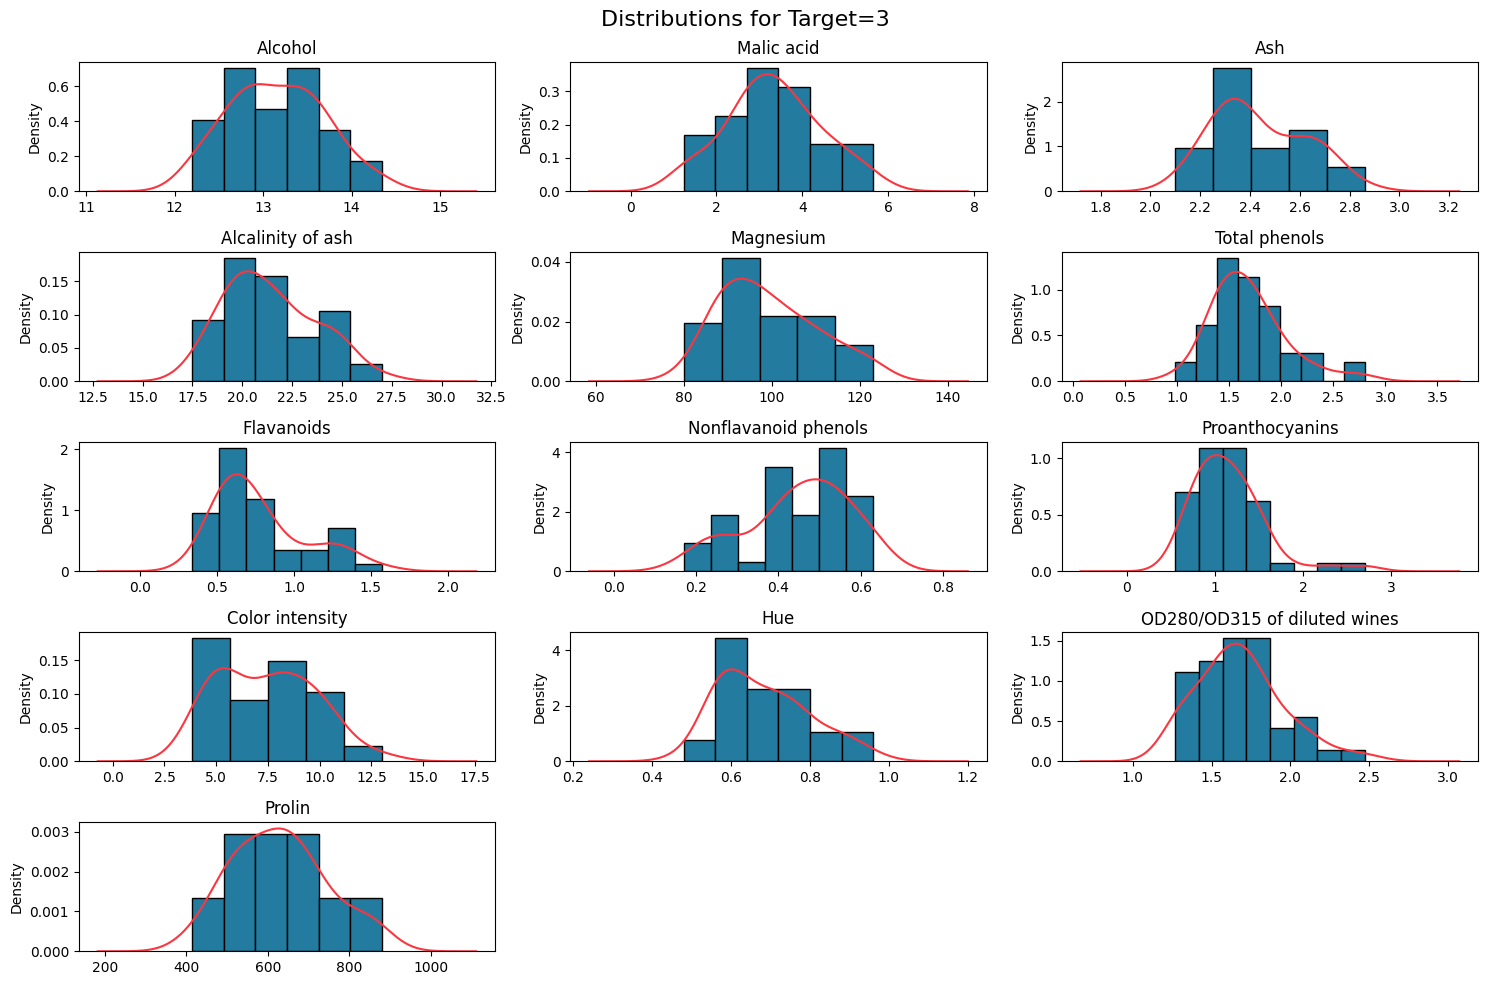
\includegraphics[width=\textwidth]{figures/Distribiutions_target3.png}
    \caption{Distributions of the considered variables for observations belonging to class 3.}
    \label{fig:distributions_target3}
\end{figure}

\begin{figure}[!htbp]
    \centering
    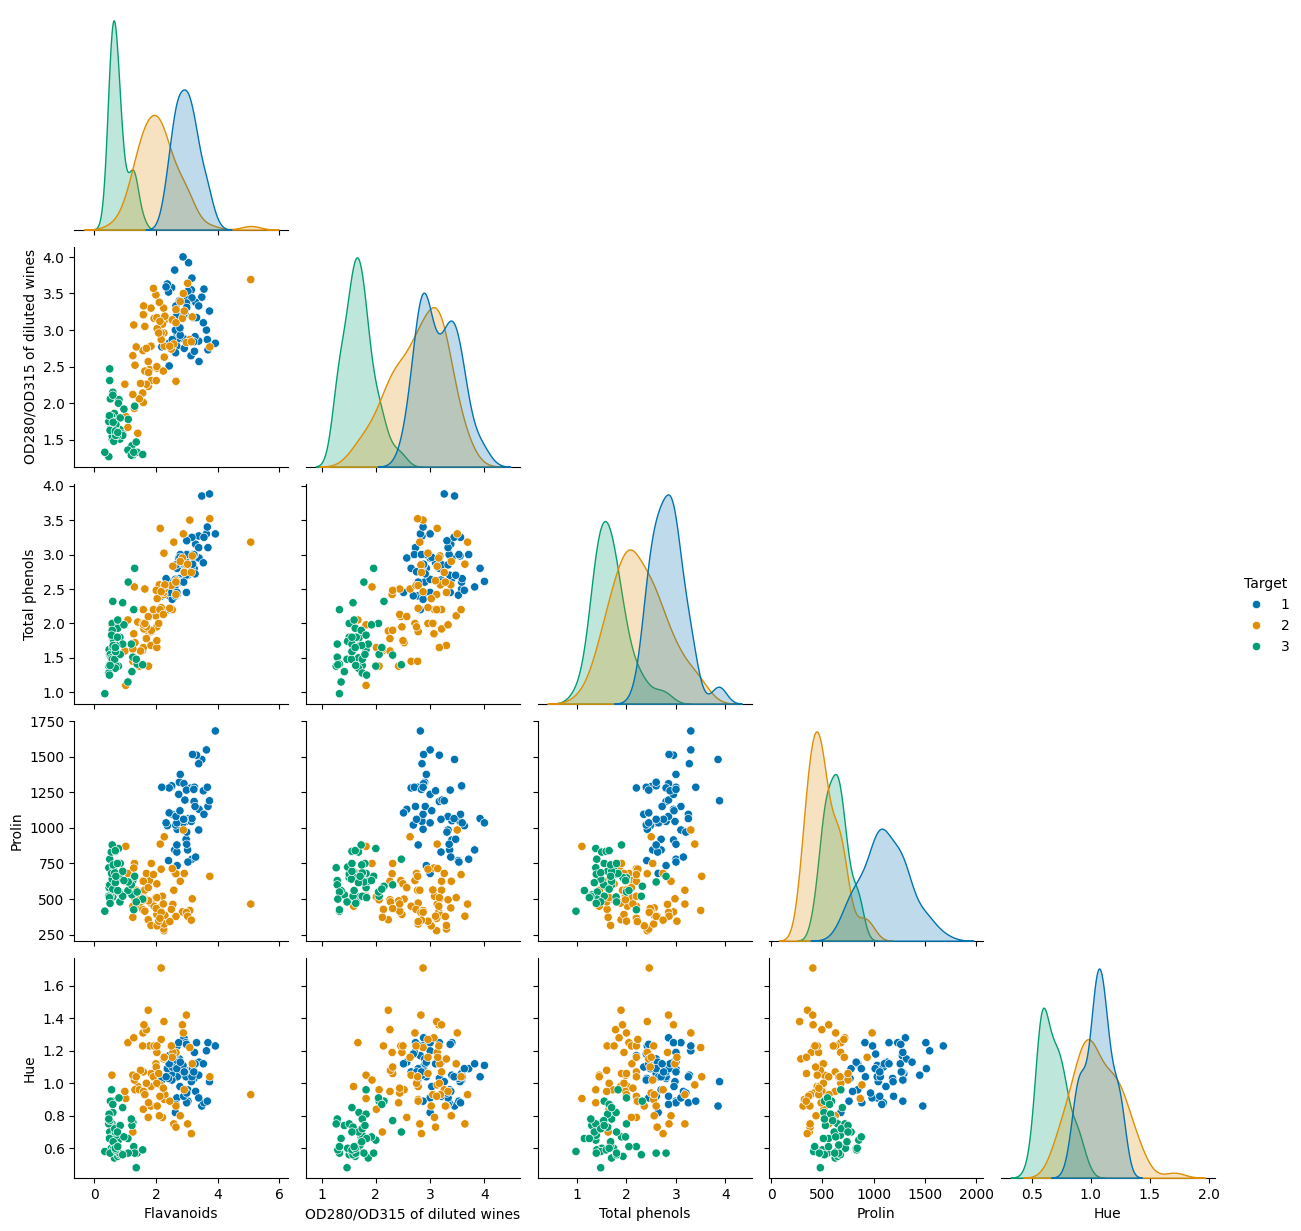
\includegraphics[width=\textwidth]{figures/pairplot.png}
    \caption{Pairplot for selected variables in the dataset.}
    \label{fig:pairplot}
\end{figure}

\FloatBarrier